% !TeX spellcheck = it_IT
\documentclass[a4paper,12pt]{article}

\usepackage{alltt, fancyvrb, url}
\usepackage{graphicx}
\usepackage{algorithmic}
\usepackage[utf8]{inputenc}
\usepackage{titling}
\usepackage{fancyhdr}
\usepackage{fontenc}
\usepackage{amsmath,mathtools,algorithm}
\usepackage{amssymb}
\usepackage{longtable}
\usepackage{setspace}
\usepackage{listings}
\usepackage{color}
\usepackage{eurosym}
\usepackage{array}
\usepackage[referable]{threeparttablex}
\usepackage{pifont}
\usepackage{siunitx}

\newcommand{\cmark}{\ding{51}}
\newcommand{\xmark}{\ding{55}}

\usepackage[italian,hidelinks]{hyperref}

\usepackage[italian]{babel}
\usepackage[italian]{cleveref}


\pretitle{%
	\begin{center}
		\LARGE
	}
\posttitle{\end{center}}


\title{\Huge \textbf{Evolutionary Cars} \\
	\vspace{10pt}
	\vspace{20pt}
}
\author{
	Gabriele Graffieti \\ \small \url{gabriele.graffieti@studio.unibo.it}
	\vspace{15pt}
	\\
	Alfredo Maffi \\ \small \url{alfredo.maffi@studio.unibo.it}
	\vspace{15pt}
	\\
	Manuel Peruzzi \\ \small \url{manuel.peruzzi@studio.unibo.it}
}

\date{}

\begin{document}

\maketitle
\pagenumbering{arabic}
\newpage
\tableofcontents
\newpage

\section{Introduzione}

Questo documento è la relazione del progetto Evolutionary Cars, realizzato per il corso di Sistemi Intelligenti Robotici, erogato dalla facoltà di Ingegneria e Scienze Informatiche dell'Università di Bologna (A.A. 2017/2018).

\section{Stato dell'arte}

\section{Architettura} \label{architecture}
In questa sezione verrà illustrata l'architettura generale del sistema. La progettazione è stata effettuata in modo da isolare gli aspetti chiave da quelli relativi all'ambiente di esecuzione. Di conseguenza, il sistema risulta suddiviso in due sottoparti principali: \emph{core} e ambiente di esecuzione. La parte core raggruppa al suo interno tutti i concetti del sistema che si rivelano indipendenti dall'ambiente nel quale esso viene eseguito. D'altro canto, la parte relativa all'ambiente di esecuzione si rivela necessaria per permettere al sistema di adattarsi ed essere eseguito in un certo ambiente, sia esso reale o virtuale. Segue una breve descrizione dei componenti del sistema.
\begin{description}
	\item[Driver Agent]: entità preposta alla guida di un'auto. Indipendentemente dall'implementazione e dalla natura del veicolo, determina la potenza del motore e la direzione di sterzata dello stesso, a partire dalle informazioni relative alla distanza dai muri del tracciato. Ogni decisione che incide sul movimento dell'auto è determinata da una rete neurale interna, i cui pesi sono regolati in modo da aderire al genotipo dell'agente.
	\item[Neural Network]: rete neurale feedforward utilizzata per pilotare un'auto. Riceve in input cinque valori di prossimità, che descrivono lo stato dell'auto in relazione ai muri del tracciato, e produce in output forza motore e direzione dello spostamento successivo. I pesi della rete sono inizialmente definiti in modo casuale, per poi essere adattati in corso d'opera in seguito all'evoluzione del genotipo corrispondente.
	\item[Genotype]: insieme di informazioni che contraddistinguono il comportamento di un'auto da un'altro. In particolare, contiene i pesi da assegnare alla \emph{neural network} di un particolare agente.
	\item[Genetic Algorithm]: algoritmo finalizzato all'evoluzione dei genotipi da una generazione alla successiva. Si compone delle fasi di selezione, crossover e mutazione, che saranno discusse nel dettaglio in \autoref{evolution}.
	\item[Controller]: può essere definito come il collante tra le parti di core e simulazione del sistema. Si occupa inizialmente di istanziare l'algoritmo genetico ed un insieme di driver agent. È responsabile dell'avvio del processo di \emph{evaluation} dei genotipi, interagendo con un componente relativo alla gestione della parte di simulazione. Al termine di tale processo viene notificato, in modo da poter poi provvedere all'avvio della fase di evoluzione, interagendo con l'algoritmo genetico.
\end{description}
In \autoref{architecture-diagram} è illustrato un diagramma che descrive, in maniera informale, l'architettura del sistema. Per quanto riguarda la parte relativa all'ambiente di esecuzione, in \autoref{simulation} verrà proposta un'infrastruttura per effettuare una simulazione del sistema.

\begin{figure}[H]
	\centering
	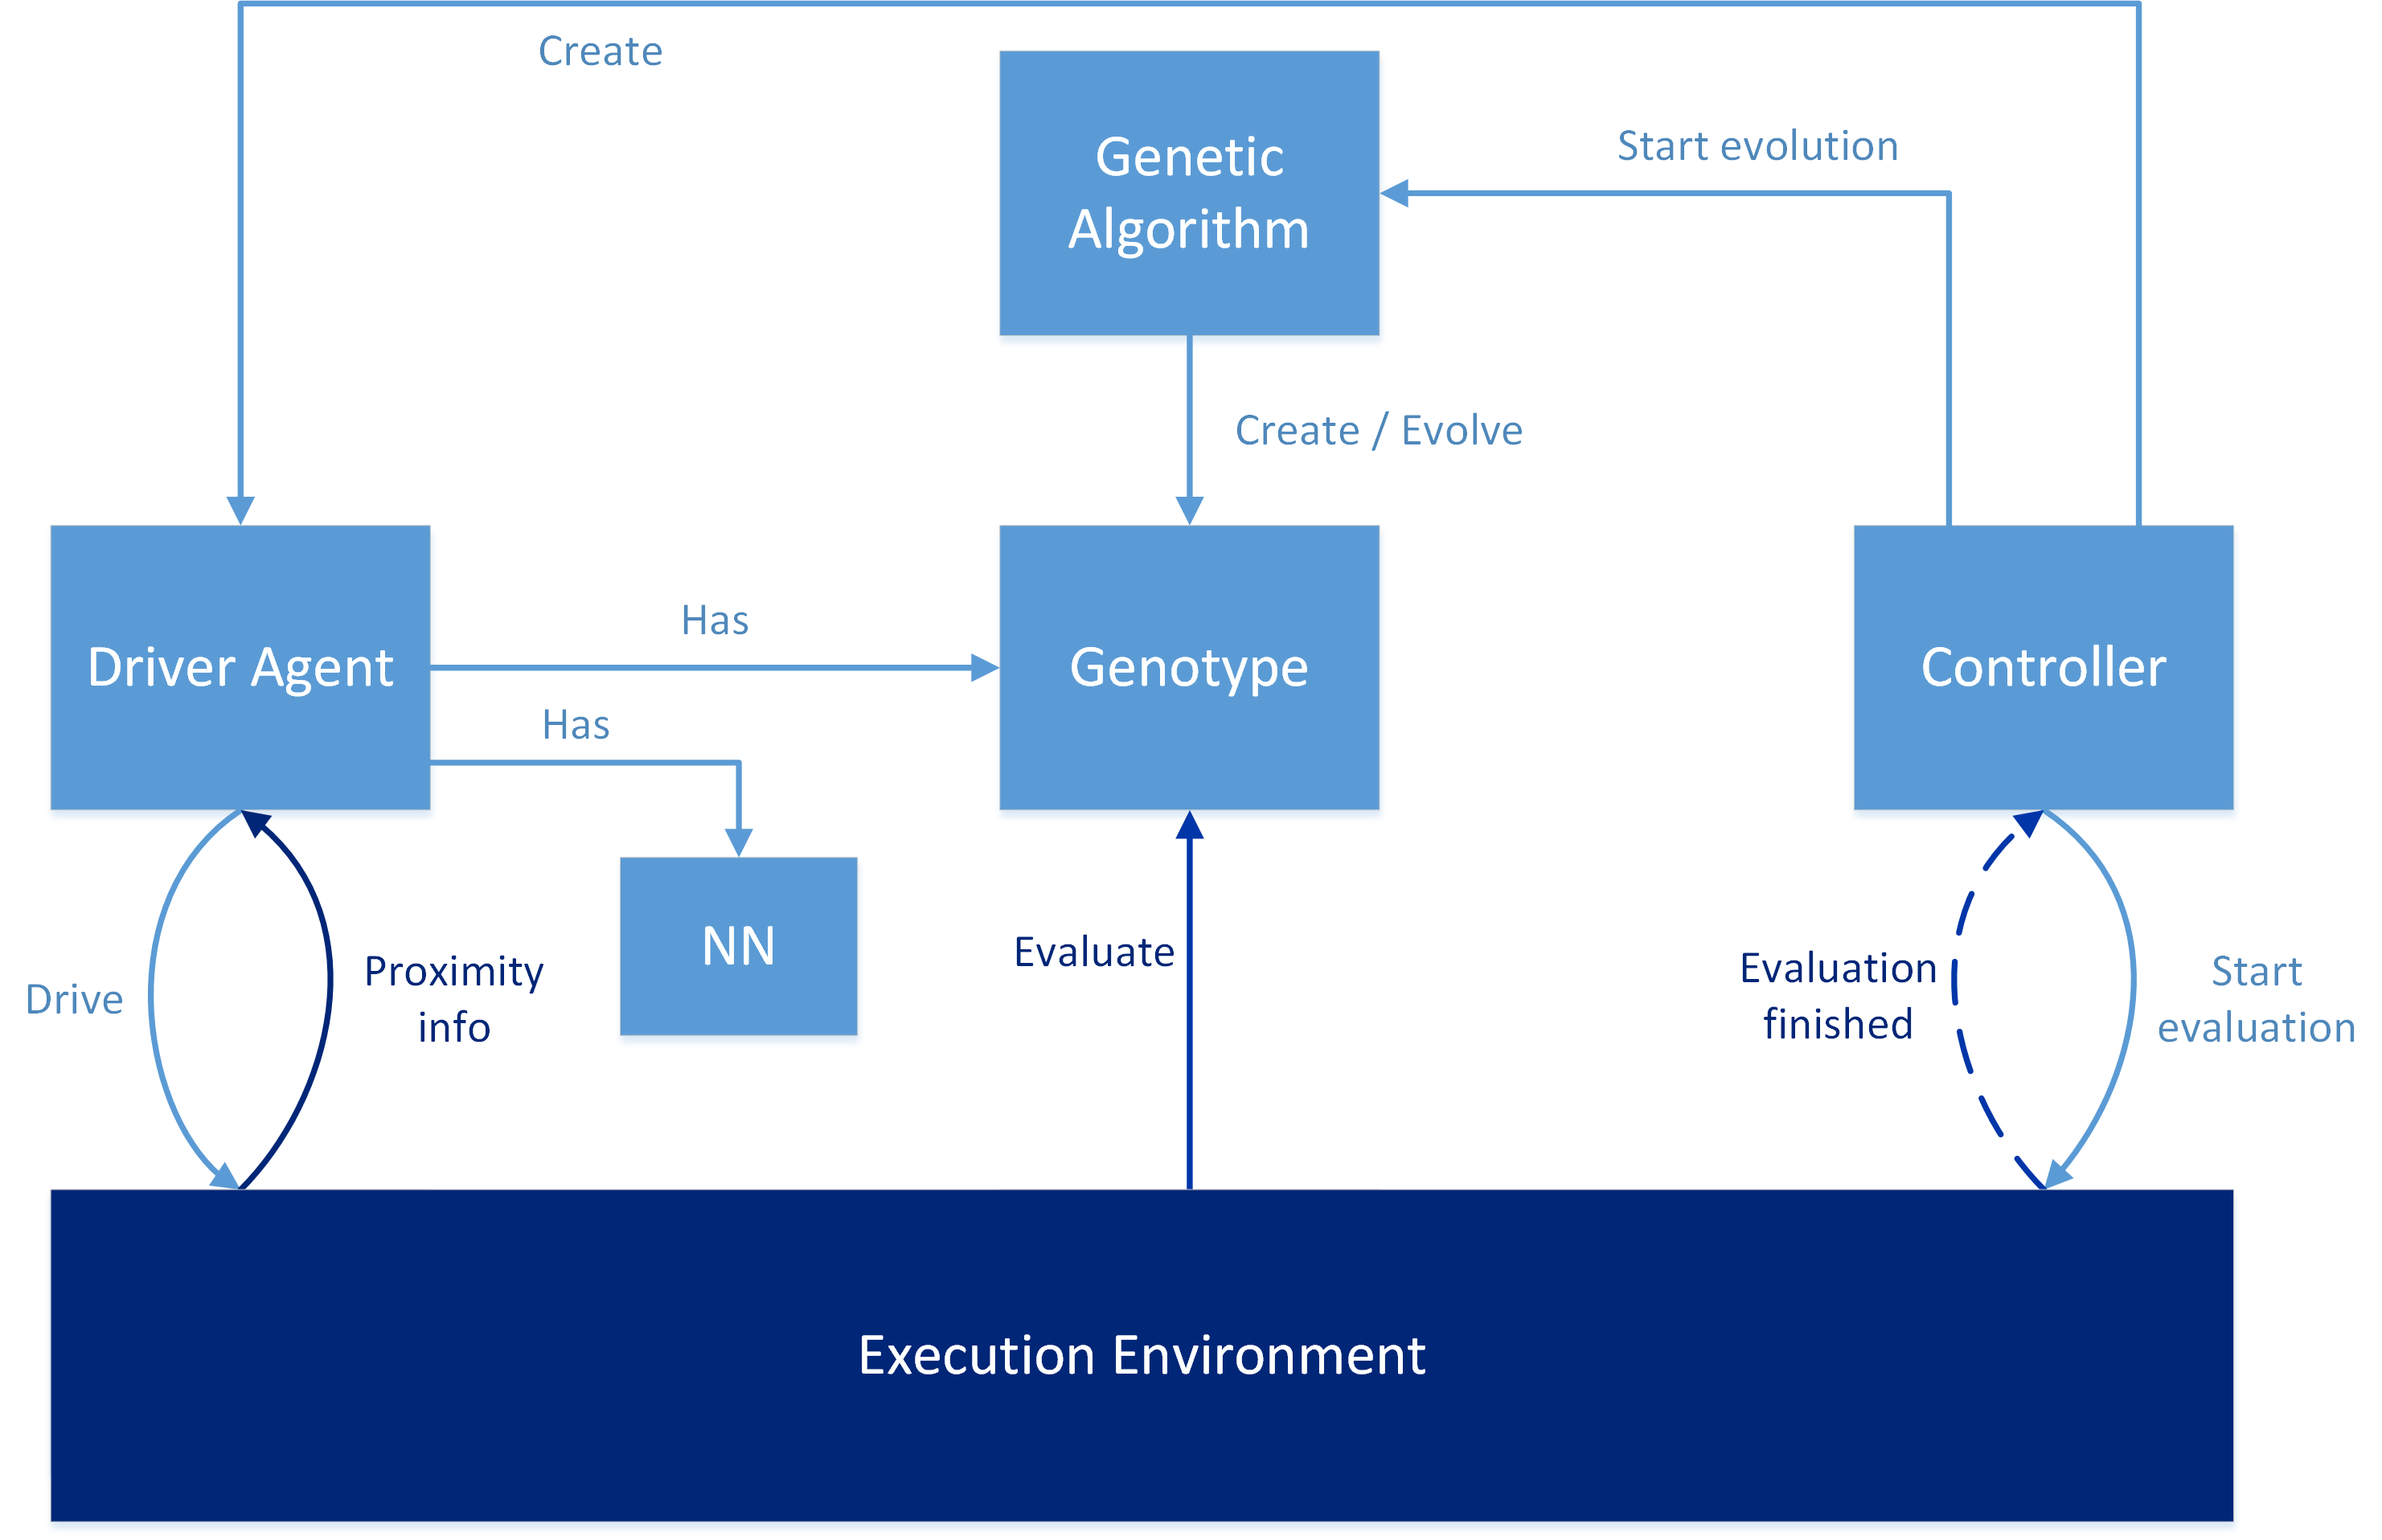
\includegraphics[width=130mm]{./img/architecture.png}
	\caption{Diagramma informale che rappresenta le relazioni tra i componenti che formano l'architettura del sistema. Nella notazione utilizzata, le frecce tratteggiate indicano una notifica dell'avvenimento di un certo evento, a differenza delle frecce continue che si riferiscono a relazioni di dipendenza. Nel diagramma sono rappresentati solamente i componenti relativi alla parte \emph{core} del sistema; quelli relativi all'ambiente di esecuzione non sono trattati in questo diagramma e sono, perciò, stati collassati nel blocco \emph{Execution Environment}.  \label{architecture-diagram}}
\end{figure}

\section{Evoluzione} \label{evolution}
% bisogna spiegare perchè l'evaluation è fatta da un componente della simulazione e non da uno del core
% oltre all'evaluation, bisogna spiegare anche il timeout

\section{Simulazione} \label{simulation}

L'architettura illustrata in \autoref{architecture} mette in evidenza i componenti principali del sistema. Come anticipato, per completare l'architettura si rivela necessaria l'aggiunta di ulteriori componenti, dipendenti dall'ambiente di esecuzione. Nel progetto in esame, si è scelto di simulare l'ambiente di esecuzione attraverso l'utilizzo di un motore grafico. Il blocco \emph{Execution Environment}, presente in \autoref{architecture-diagram}, è stato raffinato nei seguenti componenti.
\begin{description}
	\item[Car]: rappresenta un'auto. È equipaggiata con cinque sensori di prossimità in grado di percepire la distanza da eventuali ostacoli o muri. Più nello specifico, ogni sensore è posizionato secondo una certa angolazione rispetto all'asse dell'auto, da \ang{-60} fino a \ang{+60}. In questo modo è possibile effettuare una completa operazione di \emph{sensing} nella zona frontale rispetto al veicolo. Ogni auto è associata ad un \emph{Driver Agent}, al quale deve inoltrare i valori rilevati dai sensori per ottenere indicazioni sullo spostamento da effettuare. Se dai sensori viene rilevata una collisione con i muri del tracciato, l'auto si ferma immediatamente, notificando il \emph{Race Manager}.
	\item[Race Manager]: è il componente dedito all'esecuzione della fase di \emph{evaluation} di ogni generazione dell'algoritmo genetico. Più nel dettaglio, all'avvio ha il compito di creare auto e tracciato, mentre durante l'evaluation è responsabile del controllo dello stato di ogni auto. All'inizio di ogni iterazione, si occupa del riposizionamento di ogni auto all'inizio del tracciato. Al termine dell'iterazione, ovvero quando tutte le macchine hanno segnalato una collisione o hanno terminato il tracciato, provvede ad assegnare una valutazione al genotipo corrispondente ad ogni auto e a notificare il \emph{Controller}.
	\item[Track]: rappresenta il tracciato, circondato da muri, sul quale si muovono le auto. Su di esso sono disposti dei \emph{checkpoint}, utilizzabili per effettuare l'evaluation del genotipo di ogni auto. I checkpoint sono posizionati, in maniera uniforme, per tutta la lunghezza del tracciato. Il raggiungimento dell'ultimo di essi sancisce il completamento del tracciato.
\end{description}
I componenti appena descritti sono rappresentati in \autoref{simulation-diagram}, insieme all'architettura generale del sistema.

In questa sezione è stata proposta una possibile architettura per la parte del sistema relativa all'ambiente di esecuzione. L'implementazione dei componenti relativi alla parte dell'ambiente di esecuzione non può essere sviluppata in maniera generale, ma contiene, necessariamente, dei riferimenti all'ambiente stesso. In questo progetto l'ambiente di esecuzione è stato simulato tramite l'utilizzo del motore grafico \emph{Godot}\footnote{\url{https://godotengine.org/}}. Nel caso si voglia adottare un differente ambiente di esecuzione, sia reale che simulato, sarà sufficiente variare l'implementazione dei componenti \emph{Car}, \emph{Race Manager} e \emph{Track} in modo da adattarli all'ambiente scelto. Non sarà necessario apportare modifiche al \emph{core}, a patto che vengano preservate le interazioni tra le due parti del sistema, descritte nell'architettura in \autoref{architecture}.

\begin{figure}[H]
	\centering
	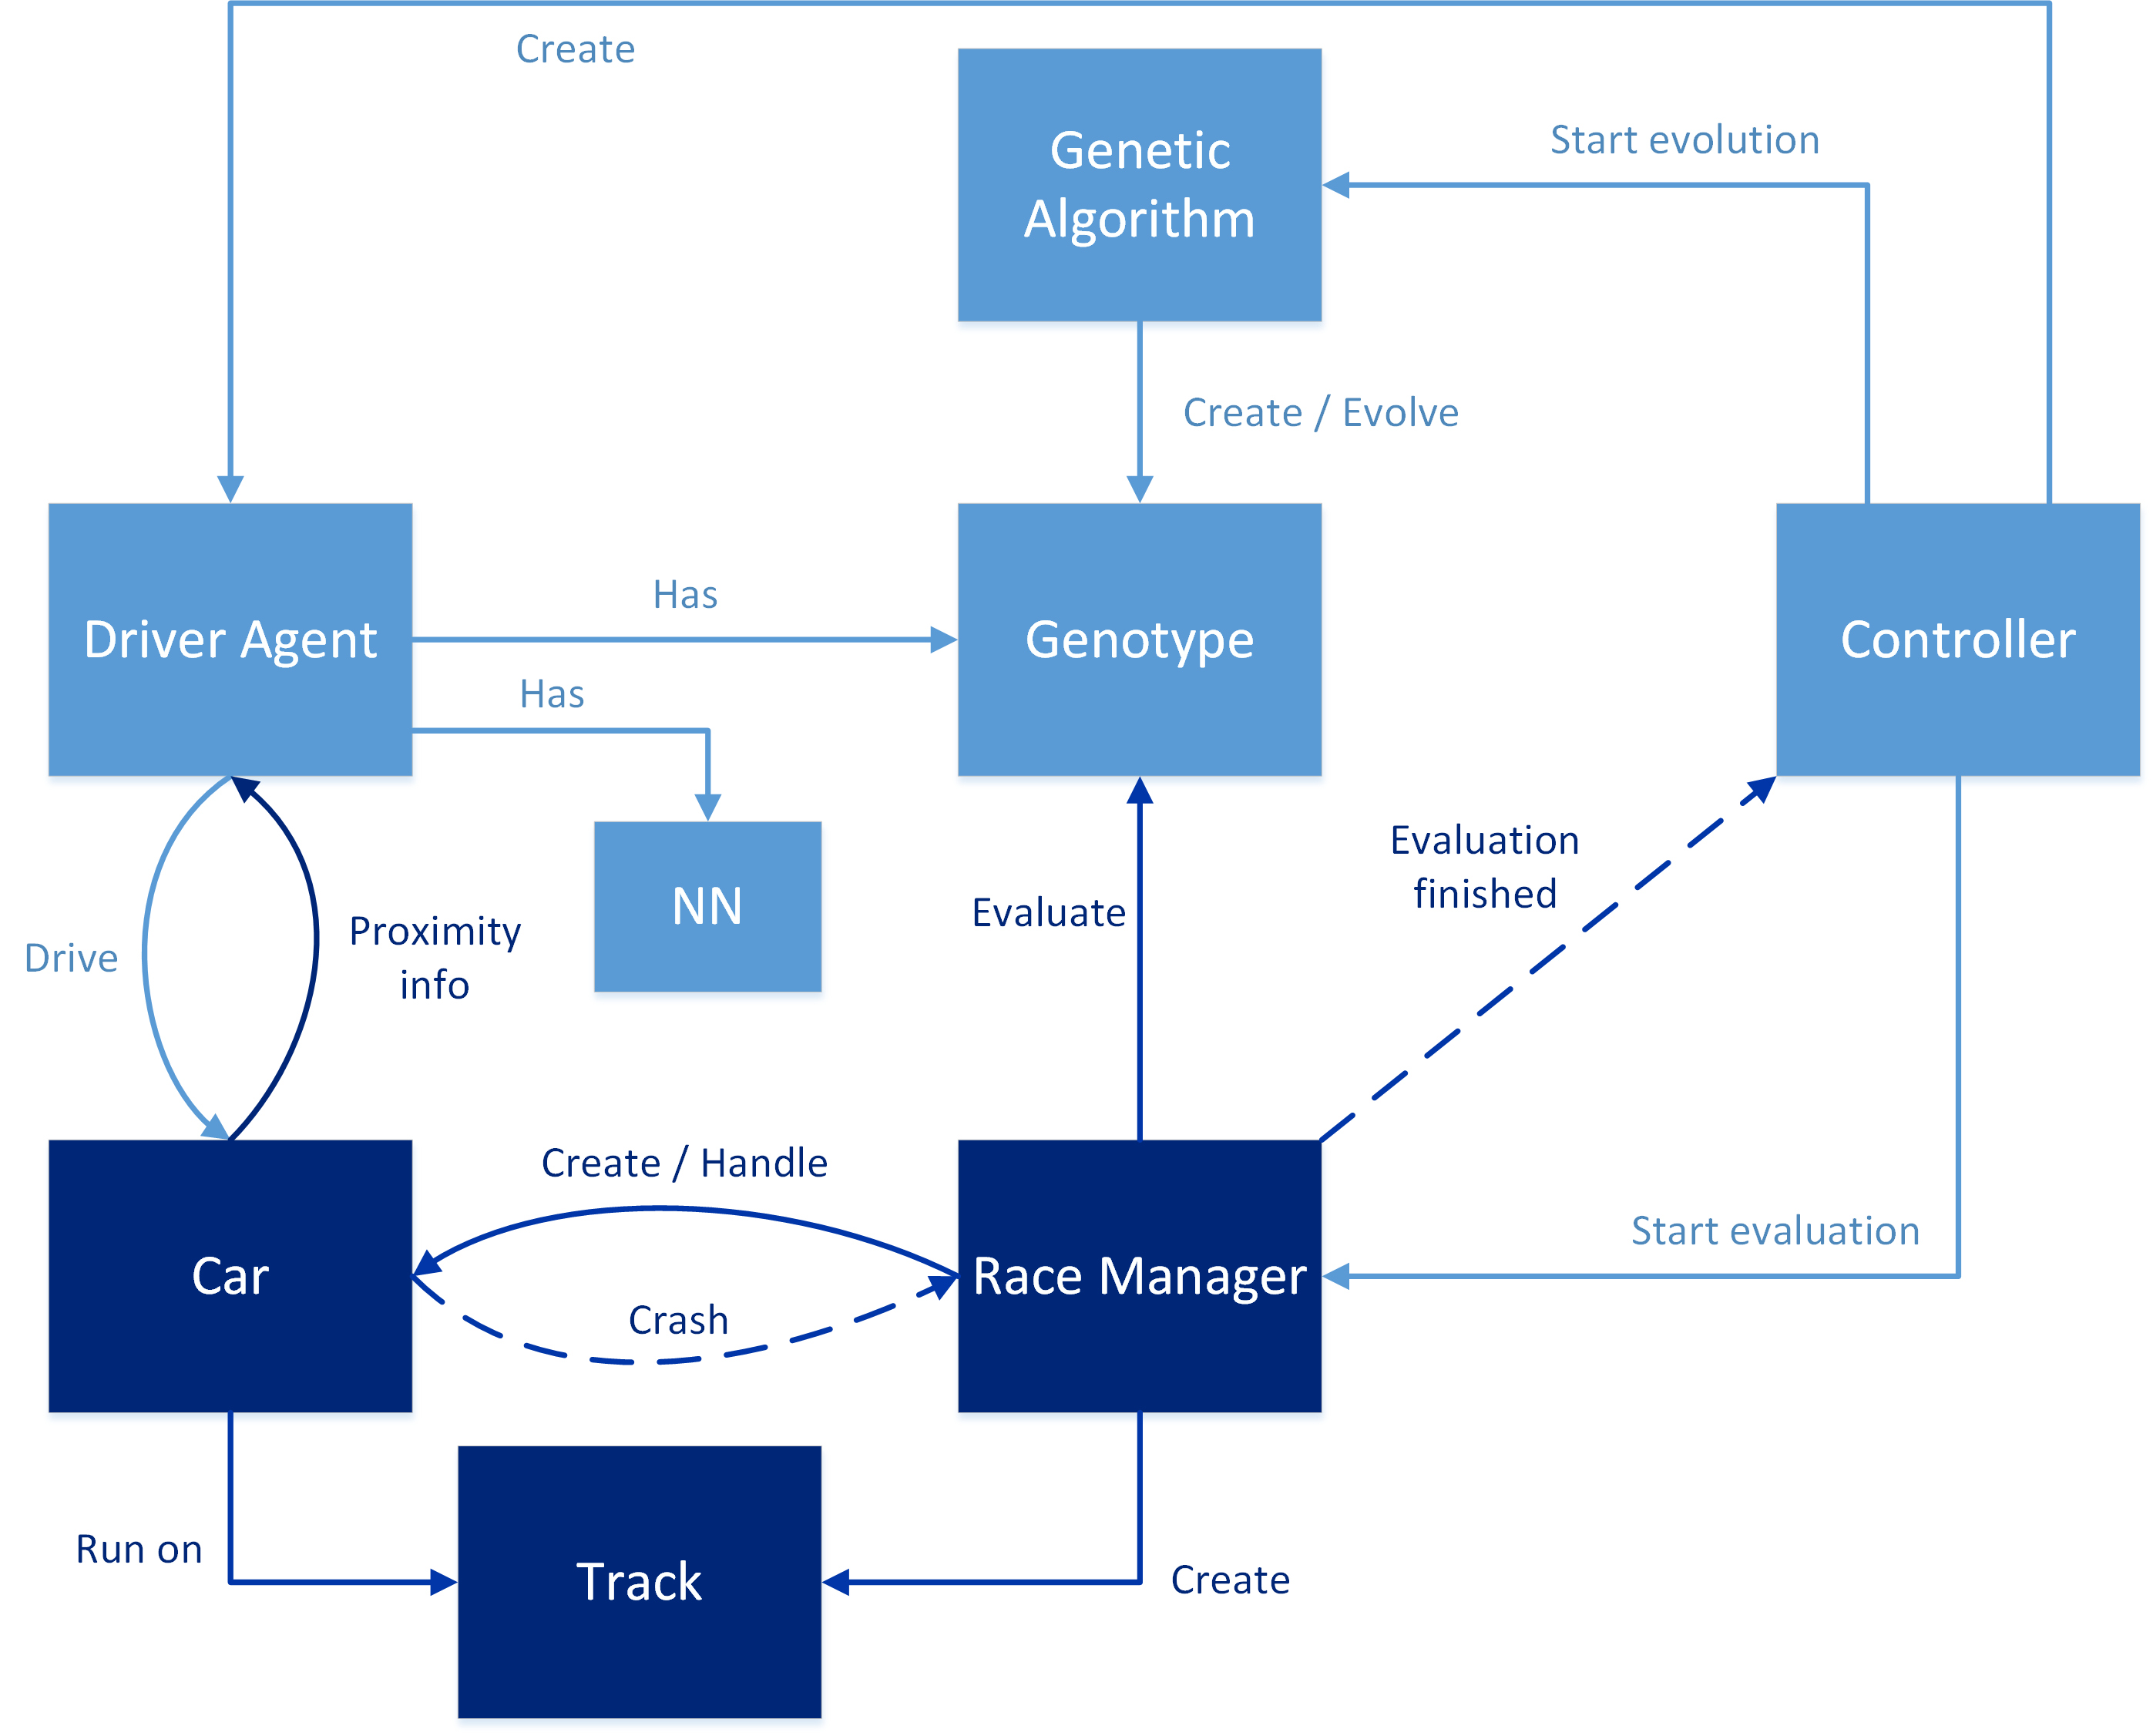
\includegraphics[width=130mm]{./img/architecture-simulation.png}
	\caption{Diagramma informale che rappresenta le relazioni tra i componenti che formano l'architettura del sistema. Nella notazione utilizzata, le frecce tratteggiate indicano una notifica dell'avvenimento di un certo evento, a differenza delle frecce continue che si riferiscono a relazioni di dipendenza. Nel diagramma i componenti caratterizzati da un colore più scuro sono quelli relativi alla simulazione, distinguibili dai restanti che costituiscono invece il \emph{core} del sistema.  \label{simulation-diagram}}
\end{figure}

\section{Risultati}

\section{Conclusioni}

\end{document}
